% Observation geometry: what decides whether a pass is seen. Schematic, not to scale.
% Built by experiments/diagrams/build_diagrams.py. Palette: Okabe-Ito.
\documentclass[border=4pt]{standalone}
\usepackage{amsmath}
\usepackage{tikz}
\usetikzlibrary{arrows.meta, calc, angles, quotes, decorations.pathmorphing}
\definecolor{orbit}{HTML}{0072B2}
\definecolor{sun}{HTML}{E69F00}
\definecolor{shadow}{HTML}{555555}
\definecolor{score}{HTML}{CC79A7}
\definecolor{bad}{HTML}{D55E00}
\definecolor{good}{HTML}{009E73}
\begin{document}
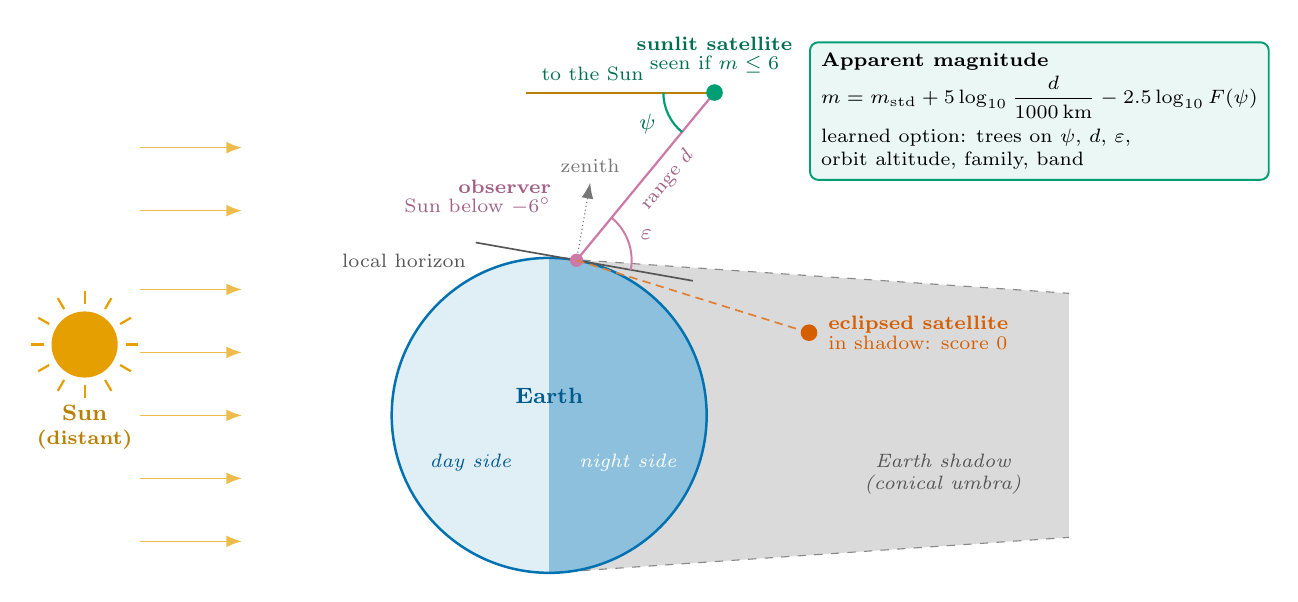
\begin{tikzpicture}[font=\footnotesize, >={Latex[length=2mm, width=1.5mm]}]
% ---------------------------------------------------------------- sunlight
\foreach \y in {-1.6, -0.8, 0, 0.8, 1.6, 2.6, 3.4}
  \draw[->, sun!70, line width=0.6pt] (-5.2,\y) -- (-3.9,\y);
\fill[sun] (-5.9,0.9) circle (0.42);
\foreach \a in {0,30,...,330}
  \draw[sun, line width=0.8pt] ($(-5.9,0.9)+(\a:0.52)$) -- ($(-5.9,0.9)+(\a:0.68)$);
\node[text=sun!80!black, font=\footnotesize\bfseries, align=center] at (-5.9,-0.15) {Sun\\[-1pt]\scriptsize(distant)};
% ---------------------------------------------------------------- Earth shadow
\fill[shadow!22] (0,2) -- (6.6,1.55) -- (6.6,-1.55) -- (0,-2) -- cycle;
\draw[shadow!70, dashed] (0,2) -- (6.6,1.55);
\draw[shadow!70, dashed] (0,-2) -- (6.6,-1.55);
\node[text=shadow, font=\scriptsize\itshape, align=center] at (5.0,-0.75) {Earth shadow\\(conical umbra)};
% ---------------------------------------------------------------- Earth, day and night
\fill[orbit!12] (0,0) circle (2);
\begin{scope}
  \clip (0,0) circle (2);
  \fill[orbit!45] (0,-2.1) rectangle (2.1,2.1);
\end{scope}
\draw[orbit, line width=0.9pt] (0,0) circle (2);
\node[text=orbit!80!black, font=\scriptsize\itshape] at (-1.0,-0.6) {day side};
\node[text=white, font=\scriptsize\itshape] at (1.0,-0.6) {night side};
\node[text=orbit!80!black, font=\footnotesize\bfseries] at (0,0.25) {Earth};
% ---------------------------------------------------------------- observer and local horizon
\coordinate (O) at (80:2);
\coordinate (Z) at (80:3.0);
\draw[shadow, line width=0.6pt] ($(O)+(-10:-1.3)$) -- ($(O)+(-10:1.5)$);
\node[shadow, font=\scriptsize, anchor=north east] at ($(O)+(-10:-1.3)+(0,-0.02)$) {local horizon};
\draw[->, shadow!80, densely dotted] (O) -- (Z) node[above, font=\scriptsize] {zenith};
\fill[score] (O) circle (2.4pt);
\node[score!80!black, font=\scriptsize\bfseries, anchor=south east, align=right] at ($(O)+(-0.2,0.45)$)
     {observer\\[-1pt]\normalfont Sun below $-6^\circ$};
% ---------------------------------------------------------------- visible satellite
\coordinate (S) at (2.1,4.1);
\draw[line width=0.8pt, score] (O) -- node[sloped, below, pos=0.55, font=\scriptsize, text=score!80!black] {range $d$} (S);
\draw[sun!80!black, line width=0.7pt] (S) -- ++(-2.4,0);
\coordinate (P) at ($(S)+(-2.4,0)$);
\pic[draw=good, line width=0.8pt, angle radius=6.5mm, "$\psi$", angle eccentricity=1.45, text=good!70!black]
    {angle = P--S--O};
\coordinate (H) at ($(O)+(-10:1.5)$);
\pic[draw=score, line width=0.7pt, angle radius=7mm, "$\varepsilon$", angle eccentricity=1.35, text=score!80!black]
    {angle = H--O--S};
\fill[good] (S) circle (3pt);
\node[good!70!black, font=\scriptsize\bfseries, anchor=south, align=center] at ($(S)+(0,0.12)$)
     {sunlit satellite\\[-1pt]\normalfont seen if $m \le 6$};
\node[good!70!black, font=\scriptsize, anchor=south] at ($(S)+(-1.55,0.03)$) {to the Sun};
% ---------------------------------------------------------------- eclipsed satellite
\coordinate (E) at (3.3,1.05);
\draw[line width=0.6pt, bad!80, densely dashed] (O) -- (E);
\fill[bad] (E) circle (3pt);
\node[bad, font=\scriptsize\bfseries, anchor=west, align=left] at ($(E)+(0.12,0.0)$)
     {eclipsed satellite\\[-1pt]\normalfont in shadow: score 0};
% ---------------------------------------------------------------- photometry box
\node[draw=good, fill=good!8, rounded corners=3pt, line width=0.7pt, align=left,
      inner sep=4pt, font=\scriptsize, anchor=north west] at (3.3,4.75)
     {\textbf{Apparent magnitude}\\[1pt]
      $m = m_\mathrm{std} + 5\log_{10}\dfrac{d}{1000\,\mathrm{km}} - 2.5\log_{10}F(\psi)$\\[3pt]
      learned option: trees on $\psi$, $d$, $\varepsilon$,\\
      orbit altitude, family, band};
\end{tikzpicture}
\end{document}
